% ====================================================================================
\chapter{从高数到约束优化}
% ====================================================================================

\section*{一把被低估的钥匙}

1755年，19岁的Joseph-Louis Lagrange给当时最伟大的数学家Leonhard Euler写了一封信，提出了一种求解变分问题的新方法。Euler收到信后大为震惊——这个方法比他自己发明的方法简洁得多。

更令人惊讶的是，Euler并没有嫉妒这个年轻人。相反，他故意推迟发表自己的工作，让Lagrange先发表。他写道："我不想在这个主题上发表任何东西，直到这位年轻人有机会发表他的发现。"

这就是Lagrange（1736--1813），一个改变了数学和物理学的人。拿破仑称他为"数学科学的高耸金字塔"。他性格温和，从不与人争论优先权。他的名言是："如果我能避免计算，我就避免"——他追求的是优雅而非繁琐。

\clarify{Lagrange虽然以法国数学家著称，但实际上出生在意大利都灵。他的原名是Giuseppe Lodovico Lagrangia。}

今天，几乎每个理工科学生都在《高等数学》或《数学分析》课上学过"拉格朗日乘子法"。但大多数人只把它当成一种解题技巧——用来应付"固定周长求最大面积"之类的考试题。

这是一个巨大的误解。

拉格朗日乘子法不是考试技巧。它是理解现代物理学、控制论、机器学习的\textbf{统一语言}。从牛顿力学到量子场论，从机器人控制到AlphaGo，背后都是同一套数学框架。

\vspace{0.5cm}
\noindent\textit{为什么你的手机能在几毫秒内规划导航路线？为什么AlphaGo能在围棋中击败人类冠军？为什么桥梁不会在正常使用中塌陷？}

\vspace{0.3cm}
这些看似毫不相关的问题，背后都藏着同一个数学工具——\textbf{拉格朗日乘子法}。

\begin{quote}
\textbf{本章目标}：让你意识到拉格朗日乘子法不是"考试技巧"，而是理解物理和AI的核心语言。读完本章，你会发现自己已经掌握了打开多扇大门的钥匙。
\end{quote}

\begin{tcolorbox}[colback=green!5, colframe=green!60!black, title=学完这章，你将能够...]
\begin{itemize}
    \item 求解带等式/不等式约束的优化问题（工程设计、资源分配）
    \item 写出任意约束优化问题的KKT条件
    \item 解释"影子价格"的经济学含义（约束放松1单位，目标改善多少？）
    \item 判断一个优化问题是否是凸问题，并利用凸性简化求解
    \item 为后续章节（力学、控制、机器学习）建立统一的数学语言
\end{itemize}
\end{tcolorbox}

% ------------------------------------------------------------------------------------
\section{问题的起点}

让我们从一个简单的问题开始：

\textbf{问题}：原点到平面$x + y + z = 1$的最短距离是多少？

数学描述：
\[
\min_{x,y,z} \quad x^2 + y^2 + z^2 \quad \text{s.t.} \quad x + y + z - 1 = 0
\]

\subsection{传统方法：代入消元}

一种"朴素"的做法是：从约束中解出$z = 1 - x - y$，代入目标函数，变成无约束问题：
\[
\min_{x,y} \quad x^2 + y^2 + (1-x-y)^2
\]

然后对$x$、$y$分别求导，令导数为零，解方程组。

这种方法对简单问题还行，但有几个致命缺陷：
\begin{itemize}
    \item 如果约束复杂（比如非线性），代入后的表达式会非常丑陋
    \item 如果有多个约束，根本没法代入消元
    \item 完全丢失了问题的结构——看不出约束在优化过程中扮演什么角色
\end{itemize}

\subsection{拉格朗日的想法}

Lagrange提出了一个天才的想法：

\textbf{与其消去约束，不如把约束"融入"目标函数。}

构造一个新函数：
\[
\Lag(x, y, z, \lambda) = (x^2 + y^2 + z^2) + \lambda(x + y + z - 1)
\]

这里$\lambda$是一个新引入的变量，叫做\textbf{拉格朗日乘子}。

然后对\textbf{所有变量}求导，令导数为零：
\begin{align}
\pd{\Lag}{x} &= 2x + \lambda = 0 \\
\pd{\Lag}{y} &= 2y + \lambda = 0 \\
\pd{\Lag}{z} &= 2z + \lambda = 0 \\
\pd{\Lag}{\lambda} &= x + y + z - 1 = 0 \quad \text{（这恰好是约束！）}
\end{align}

从前三个方程得$x = y = z = -\lambda/2$，代入第四个方程得$\lambda = -2/3$，所以$x = y = z = 1/3$。

\textbf{关键观察}：
\begin{itemize}
    \item 我们引入了一个新变量$\lambda$，变量数从3个变成4个
    \item 但同时，方程数也从0个变成4个（3个驻点方程 + 1个约束）
    \item \textbf{变量数 = 方程数}，问题变成了解方程组！
\end{itemize}

% ------------------------------------------------------------------------------------
\section{核心直觉：约束等于零，加多少倍都不影响}

为什么这个方法有效？让我们来看核心直觉。

\begin{center}
\fbox{\parbox{0.9\textwidth}{
\textbf{核心直觉}：如果$x$满足约束$g(x) = 0$，那么往目标函数里加几倍的$g(x)$，结果都不变：
\[
f(x) + \lambda \cdot g(x) = f(x) + \lambda \cdot 0 = f(x)
\]
不管$\lambda$取什么值！
}}
\end{center}

换句话说：\textbf{对于所有满足约束的点}，$f(x)$和$f(x) + \lambda g(x)$的取值\textbf{完全一样}。

那我们为什么要加这一项呢？

因为加了这一项之后，问题就从"带约束优化"变成了"无约束优化"——我们可以对所有变量自由求导了！

\begin{insightbox}
这是拉格朗日乘子法的精髓：用"加一项不改变可行点处的值"的技巧，把约束优化变成无约束优化。
\end{insightbox}

% ------------------------------------------------------------------------------------
\section{视角一：变量与方程的完美匹配}

\textbf{直觉疑问}：引入乘子$\lambda$不是把问题变复杂了吗？本来$n$个未知数，现在变成$n+m$个了！

\textbf{回答}：恰恰相反，这让问题变成了"解方程"。

\begin{center}
\begin{tabular}{c|c}
\toprule
\textbf{原始视角（难）} & \textbf{拉格朗日视角（易）} \\
\midrule
在弯曲的曲面$g(x)=0$上 & 把约束融入目标 \\
寻找$f(x)$的最低点 & 变成无约束求导 \\
\midrule
变量：$n$个 & 变量：$n + m$个 \\
$x$不能随意动，必须沿着曲面走 & $\nabla_x \Lag = 0$ 给出$n$个方程 \\
直接求导$\nabla f=0$不再适用 & $\nabla_\lambda \Lag = g(x) = 0$ 给出$m$个方程 \\
& \textbf{共$n+m$个方程！}\\
\bottomrule
\end{tabular}
\end{center}

\textbf{结论}：人类擅长解方程组（线性代数），不擅长在曲面上"走来走去"。乘子法把"带约束的优化"变成了"方程个数=未知数个数"的代数问题。

\preview{这种"变量与方程完美匹配"的思想，在第4章（力学）、第7章（机器人）中会反复出现。}

\subsection{方程计数的精确化}

让我们把上面的直觉变得更精确。考虑一般问题：$n$个变量，$m$个等式约束。

\begin{center}
\begin{tabular}{c|c|c|c}
\toprule
\textbf{方法} & \textbf{变量数} & \textbf{方程数} & \textbf{是否匹配} \\
\midrule
直接求解 & $n$个（但受$m$个约束） & $\nabla f = 0$给$n$个方程， & \\
 & & 但在约束曲面上\textbf{不适用} & $\times$ \\
\midrule
代入消元 & $n-m$个 & $n-m$个驻点方程 & $\checkmark$（但结构被破坏） \\
 & （消去$m$个） & & \\
\midrule
拉格朗日法 & $n + m$个 & $n + m$个 & $\checkmark$ \\
 & （原变量+乘子） & （$n$个驻点 + $m$个约束） & \\
\bottomrule
\end{tabular}
\end{center}

\textbf{具体到开篇例子}：
\begin{itemize}
    \item 原始：3个变量$(x,y,z)$，1个约束——无法直接求导
    \item 代入消元：2个变量$(x,y)$，2个方程$\partial/\partial x = 0, \partial/\partial y = 0$——可解但丑陋
    \item 拉格朗日：4个变量$(x,y,z,\lambda)$，4个方程——优雅且保持结构
\end{itemize}

\subsection{多个约束的情形}

当有$m$个约束$g_1(x)=0, \ldots, g_m(x)=0$时，每个约束引入一个乘子：
\[
\Lag(x, \lambda_1, \ldots, \lambda_m) = f(x) + \sum_{i=1}^{m} \lambda_i g_i(x)
\]

驻点条件变成：
\begin{align}
\nabla_x \Lag &= \nabla f + \sum_{i=1}^{m} \lambda_i \nabla g_i = 0 \quad \text{（$n$个方程）}\\
\pd{\Lag}{\lambda_i} &= g_i(x) = 0 \quad \text{（$m$个方程）}
\end{align}


\think{如果$m > n$（约束比变量还多），方程组是否一定无解？什么情况下仍有解？}


% ------------------------------------------------------------------------------------
\section{视角二：$\lambda$的物理意义——影子价格}

$\lambda$不只是数学上的"凑数工具"，它有深刻的物理/经济含义。

\subsection{思想实验}

如果我们把约束稍微放松一点，从$g(x) = 0$变成$g(x) = \epsilon$（$\epsilon$是一个很小的数），最优值会怎么变化？

\textbf{数学推导}：

新问题的拉格朗日函数是：
\[
\Lag_{new} = f(x) + \lambda(g(x) - \epsilon) = \underbrace{f(x) + \lambda g(x)}_{\Lag_{old}} - \lambda \epsilon
\]

由于$-\lambda\epsilon$对$x$来说是常数，优化$x$的结果几乎不变。但\textbf{最优值}直接改变了$\lambda\epsilon$：
\[
f^*_{new} \approx f^*_{old} - \lambda \epsilon
\]

\begin{physicalmeaning}
$\lambda$是约束的\textbf{影子价格}（Shadow Price）：
\[
\lambda = -\frac{df^*}{d\epsilon}
\]
它告诉我们：如果约束放松一点点，目标函数能改善多少。
\end{physicalmeaning}

% tikz图示：影子价格
\begin{figure}[htbp]
\centering
\begin{tikzpicture}[scale=0.9]
    \draw[thick, ->] (0,0) -- (0,4) node[left] {最优值 $f^*$};
    \draw[thick, ->] (0,0) -- (5,0) node[below] {约束松弛量 $\epsilon$};
    \draw[thick, blue] (0,3) -- (4, 1);
    \node[red] at (3, 2.8) {斜率 = $-\lambda$};
    \draw[dashed] (2,0) node[below] {$\epsilon$} -- (2,2);
    \fill[blue] (0,3) circle (2pt) node[left] {原始最优值};
    \fill[blue] (2,2) circle (2pt) node[right] {松弛后};
    \node[below] at (2.5, 0.5) {\small 松弛约束 $\to$ 目标改善$\approx \lambda \epsilon$};
\end{tikzpicture}
\caption{影子价格的含义：$\lambda$度量了约束的"代价"}
\end{figure}

\subsection{经济学例子}

假设你经营一家工厂：
\begin{itemize}
    \item 目标：最大化利润$f(x)$
    \item 约束：原材料供应有限$g(x) \leq 0$
\end{itemize}

$\lambda$告诉你：如果能多买到一吨原材料（约束放松），利润能增加多少。

如果$\lambda$很大，说明原材料是"瓶颈"，值得花大价钱去买更多；如果$\lambda$很小或为零，说明原材料不是制约因素。

\think{如果两种原材料对应的$\lambda$不同，应该优先采购哪一种？}

% ------------------------------------------------------------------------------------
\section{视角三：罚函数——从软约束到硬约束}

还有第三种理解约束优化的方式——\textbf{罚函数法}。

\subsection{基本思想}

不直接处理约束，而是给违反约束的行为"罚款"：
\[
\min_x \quad f(x) + \frac{\rho}{2} |g(x)|^2
\]

这里$\rho$是罚系数。当$\rho$很大时，任何违反约束的$x$都会被"罚"得很重，所以最优解自然会趋向于满足约束。

\subsection{机械臂的例子}

考虑一个简单的机械臂问题：
\begin{itemize}
    \item 目标：两个关节$q_1, q_2$尽量不动（$\min \frac{1}{2}(q_1^2+q_2^2)$）
    \item 约束：末端必须到达位置2（$q_1 + q_2 = 2$）
\end{itemize}

用罚函数法：
\[
\mathcal{J} = \frac{1}{2}(q_1^2+q_2^2) + \frac{\rho}{2}(q_1+q_2-2)^2
\]

由对称性$q_1 = q_2 = q$，求导可得：$q = \frac{2\rho}{1+2\rho}$

\begin{center}
\begin{tabular}{ccccc}
\toprule
罚系数$\rho$ & 关节位姿$q$ & 末端误差 & 隐含乘子$\lambda \approx \rho \cdot$误差 & 物理含义 \\
\midrule
0.5 & 0.50 & -1.00 & -0.50 & 没力气，手伸不到 \\
5 & 0.91 & -0.18 & -0.90 & 接近目标 \\
50 & 0.99 & -0.02 & -0.99 & 非常精确 \\
$\mathbf{\infty}$ & \textbf{1.00} & \textbf{0.00} & \textbf{-1.00} & \textbf{刚性约束} \\
\bottomrule
\end{tabular}
\end{center}

\begin{insightbox}
\textbf{罚函数与拉格朗日乘子的关系}：当$\rho \to \infty$时，"隐含乘子"$\rho \cdot g(x)$趋向于真实的拉格朗日乘子$\lambda$。

这说明两种方法描述的是同一个物理现实，只是视角不同：
\begin{itemize}
    \item 拉格朗日法：约束是"硬"的，$\lambda$是精确的影子价格
    \item 罚函数法：约束是"软"的，$\rho \cdot g$是近似的影子价格
\end{itemize}
\end{insightbox}

% ------------------------------------------------------------------------------------
\section{不等式约束：互补松弛}

到目前为止我们只讨论了等式约束$g(x) = 0$。但实际问题中更常见的是不等式约束$h(x) \leq 0$。

\subsection{核心问题}

等式约束很简单：约束等于零，加多少倍都不影响。但不等式约束呢？

$h(x) \leq 0$不等于零！如果$h(x) < 0$，加到目标函数里会改变结果！

\subsection{解决思路}

把问题分成两种情况：

\begin{center}
\begin{tabular}{c|c|c}
\toprule
\textbf{情况} & \textbf{约束状态} & \textbf{处理方式} \\
\midrule
$h(x^*) < 0$ & 不紧（在可行域内部） & 约束"不起作用"，当它不存在 \\
$h(x^*) = 0$ & 紧绑（恰好在边界上） & 约束"激活了"，当等式处理 \\
\bottomrule
\end{tabular}
\end{center}

\subsection{互补松弛条件}

这给出了处理不等式约束的核心条件——\textbf{互补松弛}：

\begin{center}
\fbox{\parbox{0.85\textwidth}{
\textbf{互补松弛}：$\mu \cdot h(x) = 0$

意思是：乘子$\mu$和约束值$h(x)$中，\textbf{至少有一个是零}。
}}
\end{center}

\textbf{直观理解}：

\begin{itemize}
    \item \textbf{情况A：约束不紧}（$h(x^*) < 0$）

    最优解在可行域\textbf{内部}，约束对我们没有限制。

    这时乘子$\mu$\textbf{必须为零}。为什么？如果$\mu > 0$且$h < 0$，那么$\mu h < 0$，会人为降低拉格朗日函数的值，导致解偏离真实最优。

    \item \textbf{情况B：约束紧绑}（$h(x^*) = 0$）

    最优解恰好卡在\textbf{边界上}，是约束阻止了我们继续下降。

    这时乘子$\mu$\textbf{可以大于零}。因为$h = 0$，不管$\mu$取什么值，$\mu h = 0$，不影响目标。
\end{itemize}

\textbf{一句话总结}：约束要么不起作用（$\mu=0$），要么恰好取等（$h=0$）。不可能同时$\mu > 0$且$h < 0$。

\clarify{互补松弛条件的名字来源：$\mu$和$h$像"互补"的关系，一个非零另一个就必须是零。}

% ------------------------------------------------------------------------------------
\section{完整图景：KKT条件}

现在让我们把所有内容整合起来。对于一般的约束优化问题：
\[
\min_x f(x) \quad \text{s.t.} \quad g_i(x) = 0, \; h_j(x) \leq 0
\]

最优解必须满足以下条件（KKT条件）：

\begin{enumerate}
    \item \textbf{驻点条件}：$\nabla f + \sum_i \lambda_i \nabla g_i + \sum_j \mu_j \nabla h_j = 0$
    \item \textbf{原始可行}：$g_i(x) = 0$，$h_j(x) \leq 0$
    \item \textbf{对偶可行}：$\mu_j \geq 0$（不等式约束的乘子非负）
    \item \textbf{互补松弛}：$\mu_j h_j(x) = 0$
\end{enumerate}

\begin{keyidea}[KKT条件的输入与输出——大白话版]
\textbf{问题}：我有一个优化问题，想找最优解$x^*$。KKT条件怎么帮我？

\textbf{输入}：
\begin{itemize}
    \item 目标函数$f(x)$（你想最小化什么）
    \item 等式约束$g_i(x) = 0$（必须精确满足的条件）
    \item 不等式约束$h_j(x) \leq 0$（必须满足的上界）
\end{itemize}

\textbf{输出}：
\begin{itemize}
    \item 候选最优点$x^*$
    \item 拉格朗日乘子$\lambda_i^*, \mu_j^*$（约束的"价格"）
\end{itemize}

\textbf{如何使用？}
\begin{enumerate}
    \item \textbf{求解}：联立4个KKT条件，解出$(x^*, \lambda^*, \mu^*)$
    \item \textbf{验证}：检查解是否满足所有条件
    \item \textbf{理解}：$\lambda^*$告诉你约束放松一点会怎样
\end{enumerate}

\textbf{关键提醒}：KKT条件是最优解的\textbf{必要条件}。满足KKT的点是"候选最优点"，但还需要检查是否真的是极小值（而非极大值或鞍点），这就需要二阶条件（见扩展阅读）。对于\textbf{凸优化}问题，KKT条件同时是\textbf{充分条件}——满足KKT就一定是全局最优！
\end{keyidea}

\storynote{Karush, Kuhn \& Tucker}{
有趣的是，William Karush在1939年的硕士论文中就发现了这些条件，但当时没有发表。Harold Kuhn和Albert Tucker在1951年独立重新发现并发表。数学界有时就是这样——伟大的发现可能被遗忘在某个抽屉里。
}

% ------------------------------------------------------------------------------------
% 代码演示结果
\begin{figure}[htbp]
\centering
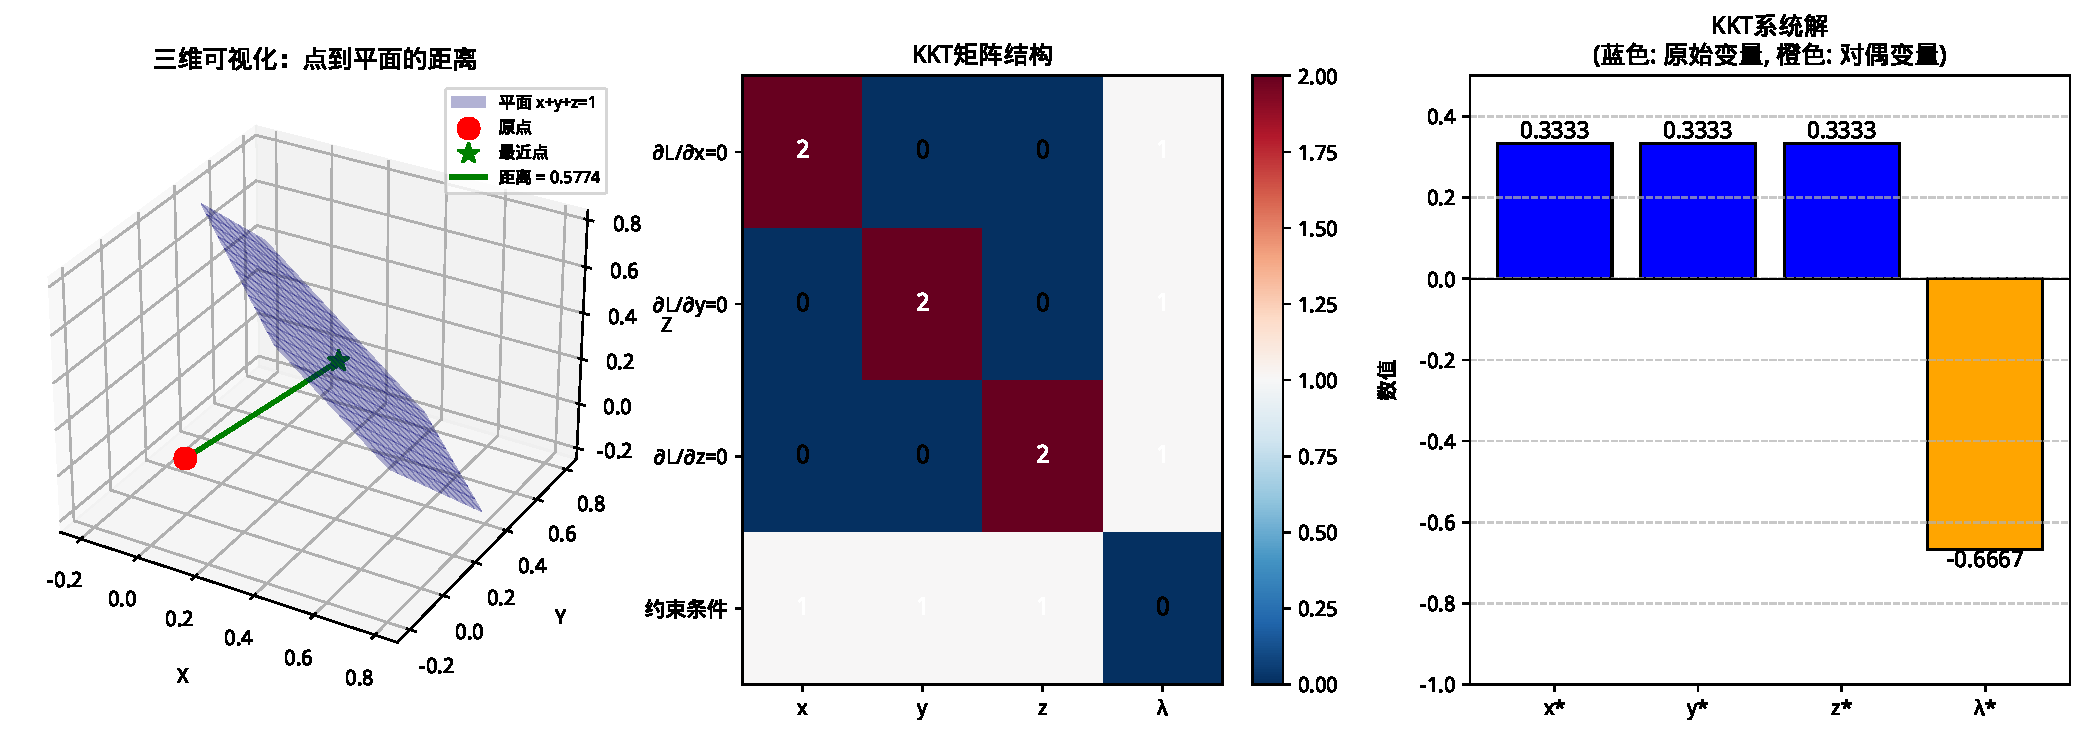
\includegraphics[width=0.85\textwidth]{figs_chap01/kkt_visualization.pdf}
\caption{KKT系统的可视化（1行3列）。\textbf{左图}：3D几何——蓝色平面为约束$x+y+z=1$，红点为原点，绿色星号为最近点，连线表示最短距离；\textbf{中图}：KKT矩阵结构热力图——矩阵有鞍点结构，对角块来自目标函数Hessian（$2I$），非对角块来自约束梯度；\textbf{右图}：KKT系统的解——蓝色柱子为原始变量$(x^*,y^*,z^*)=(1/3,1/3,1/3)$，橙色柱子为拉格朗日乘子$\lambda^*=-2/3$（负号表示约束放松会减小目标值）。}
\label{fig:chap01_kkt}
\end{figure}

\begin{figure}[htbp]
\centering
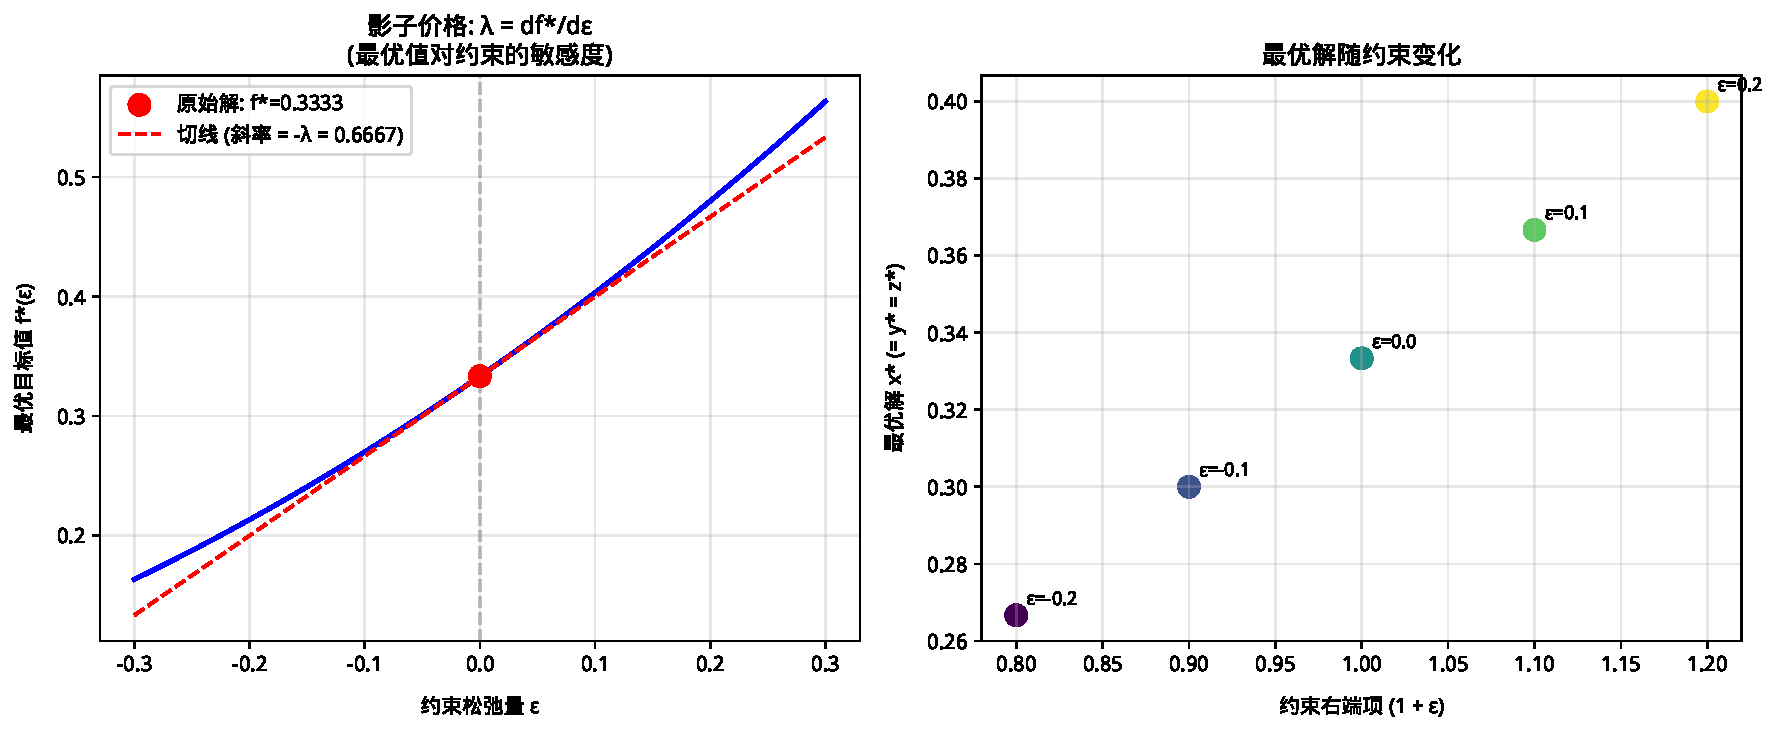
\includegraphics[width=0.85\textwidth]{figs_chap01/shadow_price.pdf}
\caption{牛顿法求解非线性约束优化的收敛过程。通过迭代求解KKT系统，算法从初始点快速收敛到约束曲面上的最优解，展示了二次收敛的特性。}
\label{fig:chap01_newton}
\end{figure}

\textbf{代码验证}：使用Python求解开篇例子的KKT系统，得到$(x^*, y^*, z^*, \lambda^*) = (1/3, 1/3, 1/3, -2/3)$，与手算结果完全一致。

% ------------------------------------------------------------------------------------
\section{本章小结}

本章我们从三个视角理解了拉格朗日乘子法：

\begin{enumerate}
    \item \textbf{代数视角}：引入乘子$\lambda$，让"变量数 = 方程数"，把约束优化变成解方程组

    \item \textbf{经济视角}：$\lambda$是约束的"影子价格"——放松约束能带来多少收益

    \item \textbf{罚函数视角}：约束可以"软化"为罚项，$\rho \to \infty$时趋向硬约束
\end{enumerate}

\begin{physicalmeaning}
本章的核心信息：$\lambda$是约束的\textbf{影子价格}——它告诉我们放松约束能带来多少收益。这个概念会贯穿全书：
\begin{itemize}
    \item 第4章：$\lambda$ = 约束力（杆的张力、支持力）
    \item 第7章：$\lambda$ = 接触力
    \item 第8章：$\lambda(t)$ = 协态变量（未来代价对当前状态的敏感度）
    \item 第9章：$\lambda$ = 反向传播中的误差信号
    \item 第10章：$\lambda$ = 值函数 $V(s)$
\end{itemize}
\end{physicalmeaning}


\section*{扩展阅读：二阶条件与正定性}
\addcontentsline{toc}{section}{扩展阅读：二阶条件与正定性}

驻点条件只告诉我们"候选点"，但无法区分极小、极大和鞍点。这就像知道山路的坡度为零，但不知道是在山顶、山谷、还是马鞍形的山口。

\subsubsection{先回顾：一维情况}

在一维微积分中，判断极值很简单：
\begin{itemize}
    \item $f''(x^*) > 0$ $\Rightarrow$ 极小（曲线向上弯）
    \item $f''(x^*) < 0$ $\Rightarrow$ 极大（曲线向下弯）
    \item $f''(x^*) = 0$ $\Rightarrow$ 需要更高阶信息
\end{itemize}

二阶导数的符号告诉我们：在驻点附近，函数是"碗形"还是"倒碗形"。

\subsubsection{多维情况：Hessian矩阵}

当$x \in \R^n$时，二阶导数变成了一个$n \times n$的矩阵——\textbf{Hessian矩阵}：
\[
\nabla^2 f = \begin{pmatrix}
\frac{\partial^2 f}{\partial x_1^2} & \frac{\partial^2 f}{\partial x_1 \partial x_2} & \cdots \\
\frac{\partial^2 f}{\partial x_2 \partial x_1} & \frac{\partial^2 f}{\partial x_2^2} & \cdots \\
\vdots & \vdots & \ddots
\end{pmatrix}
\]

问题来了：一维的"正"或"负"，在多维该怎么推广？

\subsubsection{正定与负定：多维的"碗形"与"倒碗形"}

关键思想是看\textbf{沿任意方向走，函数怎么变化}。

在驻点$x^*$附近，沿方向$v$走一小步$\epsilon$，函数值的变化（用泰勒展开）是：
\[
f(x^* + \epsilon v) - f(x^*) \approx \underbrace{\epsilon \nabla f \cdot v}_{=0,\text{因为是驻点}} + \frac{\epsilon^2}{2} v^T H v
\]

所以二阶变化完全由$v^T H v$决定！

\begin{center}
\fbox{\parbox{0.9\textwidth}{
\textbf{正定}：对所有非零方向$v$，都有$v^T H v > 0$

\textbf{含义}：不管往哪个方向走，函数值都会\textbf{增加}——这是一个"碗底"。
}}
\end{center}

\begin{center}
\fbox{\parbox{0.9\textwidth}{
\textbf{负定}：对所有非零方向$v$，都有$v^T H v < 0$

\textbf{含义}：不管往哪个方向走，函数值都会\textbf{减少}——这是一个"山顶"。
}}
\end{center}

\begin{center}
\fbox{\parbox{0.9\textwidth}{
\textbf{不定}：有些方向$v^T H v > 0$，有些方向$v^T H v < 0$

\textbf{含义}：某些方向上升，某些方向下降——这是一个"马鞍"。
}}
\end{center}

\textbf{具体例子}：考虑二维函数在原点的Hessian。

\begin{enumerate}
    \item $f(x,y) = x^2 + y^2$（碗形）
    \[
    H = \begin{pmatrix} 2 & 0 \\ 0 & 2 \end{pmatrix}, \quad v^T H v = 2v_1^2 + 2v_2^2 > 0 \quad \text{（正定）}
    \]

    \item $f(x,y) = -x^2 - y^2$（倒碗形）
    \[
    H = \begin{pmatrix} -2 & 0 \\ 0 & -2 \end{pmatrix}, \quad v^T H v = -2v_1^2 - 2v_2^2 < 0 \quad \text{（负定）}
    \]

    \item $f(x,y) = x^2 - y^2$（马鞍形）
    \[
    H = \begin{pmatrix} 2 & 0 \\ 0 & -2 \end{pmatrix}, \quad v^T H v = 2v_1^2 - 2v_2^2 \quad \text{（不定）}
    \]
    沿$x$方向（$v=(1,0)$）上升，沿$y$方向（$v=(0,1)$）下降。
\end{enumerate}

\subsubsection{如何判断正定性？}

实际操作中，不需要检验所有方向。有几个等价条件：

\begin{center}
\begin{tabular}{c|c}
\toprule
\textbf{判定方法} & \textbf{正定的条件} \\
\midrule
特征值 & 所有特征值 $> 0$ \\
顺序主子式 & 所有顺序主子式 $> 0$（Sylvester准则） \\
Cholesky分解 & 能成功分解为$H = LL^T$（$L$是下三角） \\
\bottomrule
\end{tabular}
\end{center}

\clarify{对于负定，只需检验$-H$是否正定。对于半正定（$v^T H v \geq 0$），特征值可以包含零。}

\subsubsection{约束优化的二阶条件}

现在回到约束优化。难点在于：我们只能在\textbf{约束曲面上}移动，不是整个空间。

定义\textbf{约束Hessian}（拉格朗日函数对$x$的二阶导）：
\[
H = \nabla^2_{xx} \Lag = \nabla^2 f + \sum_i \lambda_i \nabla^2 g_i
\]

\textbf{关键区别}：不需要$H$在整个空间上正定，只需要在\textbf{切空间}上正定！

切空间是什么？就是沿着约束曲面能走的方向，即满足$\nabla g_i \cdot v = 0$的所有$v$。

\begin{physicalmeaning}
\textbf{约束优化的二阶充分条件}：

设$x^*$是满足一阶条件（KKT条件）的点。如果对所有满足$\nabla g_i(x^*) \cdot v = 0$的非零方向$v$，都有
\[
v^T H v > 0
\]
则$x^*$是严格局部极小点。
\end{physicalmeaning}

\textbf{直观理解}：我们只关心"能走的方向"。即使某些方向上$H$是负的，只要那些方向被约束禁止了，就不影响极小性。

\textbf{例子}：考虑$\min x^2 - y^2$ s.t. $y = 0$。

无约束时，原点是鞍点（$H$不定）。但加上约束$y=0$后，切空间只有$x$方向，而沿$x$方向$H$是正的！所以在约束下，原点是极小点。



\subsection{矩阵形式（进阶）}

驻点条件可以写成紧凑的矩阵形式：
\[
\begin{pmatrix} \nabla f \\ g \end{pmatrix} + \begin{pmatrix} (\nabla g)^T \\ 0 \end{pmatrix} \lambda = 0
\]

或者更对称地，定义增广系统：
\[
\begin{pmatrix} \nabla^2_{xx}\Lag & (\nabla g)^T \\ \nabla g & 0 \end{pmatrix} \begin{pmatrix} \Delta x \\ \lambda \end{pmatrix} = -\begin{pmatrix} \nabla_x \Lag \\ g \end{pmatrix}
\]

这正是牛顿法求解约束优化的核心迭代格式（KKT系统）。左边的大矩阵叫做\textbf{KKT矩阵}。

\preview{这个矩阵结构会在第7章（机器人动力学）以"质量矩阵+约束雅可比"的形式再次出现。}

% ------------------------------------------------------------------------------------
\section{习题}

\paragraph{计算题}

\begin{enumerate}
    \item 对于约束$g_1(x,y,z) = x^2 + y^2 + z^2 - 1$（单位球面）和$g_2(x,y,z) = x + y - z$（平面），写出雅可比矩阵$\nabla g$，并验证它是$2 \times 3$的矩阵。
    
    \item 考虑问题$\min (x-1)^2 + (y-1)^2$ s.t. $x + y = 1$。
    \begin{enumerate}
        \item 写出拉格朗日函数$\Lag(x, y, \lambda)$
        \item 写出KKT矩阵，并验证它是$3 \times 3$的
        \item 直接求解KKT系统，得到$(x^*, y^*, \lambda^*)$
    \end{enumerate}
    
    \item 对于$2 \times 2$的KKT矩阵$K = \begin{pmatrix} 2 & 1 \\ 1 & 0 \end{pmatrix}$，计算其特征值，验证$K$是不定的（有正有负的特征值）。
\end{enumerate}

\paragraph{编程题}

\begin{enumerate}
    \setcounter{enumi}{3}
    \item 用Python/NumPy直接求解开篇例子的KKT系统：
    \[
    \begin{pmatrix} 
    2 & 0 & 0 & 1 \\
    0 & 2 & 0 & 1 \\
    0 & 0 & 2 & 1 \\
    1 & 1 & 1 & 0
    \end{pmatrix}
    \begin{pmatrix} x \\ y \\ z \\ \lambda \end{pmatrix} = 
    \begin{pmatrix} 0 \\ 0 \\ 0 \\ 1 \end{pmatrix}
    \]
    用\texttt{numpy.linalg.solve}求解，并与手算结果$(1/3, 1/3, 1/3, -2/3)$对比。
    
    \item 实现牛顿法求解非线性约束问题$\min x^2 + y^2$ s.t. $x^2 + xy + y^2 = 1$：
    \begin{enumerate}
        \item 写出KKT方程组（残差$r$）
        \item 写出KKT矩阵（残差对$(x,y,\lambda)$的雅可比）
        \item 从初始点$(1, 0, 0)$开始迭代，观察收敛过程
    \end{enumerate}
    
    \item 做实验：生成随机的正定矩阵$H$和随机的约束雅可比$A$，构造KKT矩阵$K = \begin{pmatrix} H & A^T \\ A & 0 \end{pmatrix}$。计算$K$的特征值，验证：（a）$K$总是不定的；（b）正特征值的个数等于$H$的维度，负特征值的个数等于$A$的行数。
\end{enumerate}

\paragraph{思考题}

\begin{enumerate}
    \setcounter{enumi}{6}
    \item KKT矩阵的右下角为什么是零块？如果约束函数$g$依赖于$\lambda$，会发生什么？（提示：约束的物理意义）
    
    \item 当约束数$m$远小于变量数$n$时，为什么用Schur补方法（先解$m \times m$的小系统）比直接解$(n+m) \times (n+m)$的大系统更高效？估算两种方法的计算复杂度。
    
    \item 在机器人动力学中，KKT矩阵以"质量矩阵+约束雅可比"的形式出现。猜测：$H$对应什么物理量？$\nabla g$对应什么？$\lambda$的物理意义是什么？（提示：第7章会详细讨论）
\end{enumerate}

% ------------------------------------------------------------------------------------
\section*{扩展阅读：什么是凸优化？}
\addcontentsline{toc}{section}{扩展阅读：凸优化}

在本章我们学习了约束优化的一般理论。但有一类特殊的优化问题——\textbf{凸优化}——具有非常好的性质，在机器学习和工程中应用极其广泛。

\subsection*{凸集与凸函数}

\begin{definition}[凸集]
一个集合$\mathcal{C}$是\textbf{凸集}，如果对于$\mathcal{C}$中任意两点$x, y$，连接它们的线段也完全在$\mathcal{C}$内：
\[
\forall x, y \in \mathcal{C}, \forall \theta \in [0,1]: \quad \theta x + (1-\theta)y \in \mathcal{C}
\]
\end{definition}

\begin{figure}[htbp]
\centering
\begin{tikzpicture}[scale=0.8]
    % 凸集
    \begin{scope}[shift={(0,0)}]
        \draw[thick, fill=blue!15] (0,0) ellipse (1.5cm and 1cm);
        \fill (0.5,0.3) circle (2pt) node[above] {$x$};
        \fill (-0.7,-0.2) circle (2pt) node[below] {$y$};
        \draw[red, thick] (0.5,0.3) -- (-0.7,-0.2);
        \node at (0,-1.5) {凸集 $\checkmark$};
    \end{scope}

    % 非凸集
    \begin{scope}[shift={(5,0)}]
        \draw[thick, fill=red!15] plot[smooth cycle] coordinates {(0,1) (1.2,0.5) (1,-0.5) (0.3,-0.8) (-0.5,-0.3) (-1,0.3) (-0.3,0.8)};
        \fill (0.8,0.3) circle (2pt) node[above] {$x$};
        \fill (-0.6,0.2) circle (2pt) node[above] {$y$};
        \draw[red, thick, dashed] (0.8,0.3) -- (-0.6,0.2);
        \node at (0,-1.5) {非凸集 $\times$};
    \end{scope}
\end{tikzpicture}
\caption{凸集的直观理解：线段不会``跑出去''}
\end{figure}

\begin{definition}[凸函数]
函数$f: \R^n \to \R$是\textbf{凸函数}，如果它的图形``向下弯曲''：
\[
f(\theta x + (1-\theta)y) \leq \theta f(x) + (1-\theta)f(y), \quad \forall \theta \in [0,1]
\]
等价地，$f$是凸函数当且仅当它的Hessian矩阵半正定：$\nabla^2 f \succeq 0$。
\end{definition}

\textbf{直观理解}：凸函数的图像像一个``碗''——任意两点之间的弦总在曲线上方。

\begin{example}[常见凸函数]
\begin{itemize}
    \item \textbf{线性函数}：$f(x) = a^T x + b$（既是凸函数也是凹函数）
    \item \textbf{二次函数}：$f(x) = \frac{1}{2}x^T Q x + b^T x$，当$Q \succeq 0$时是凸函数
    \item \textbf{范数}：$f(x) = \|x\|_p$（任何$p \geq 1$）
    \item \textbf{指数函数}：$f(x) = e^x$
    \item \textbf{负对数}：$f(x) = -\log x$（$x > 0$）
    \item \textbf{交叉熵损失}：深度学习中常用的损失函数
\end{itemize}
\end{example}

\subsection*{凸优化问题的定义}

\begin{definition}[凸优化问题]
一个优化问题是\textbf{凸优化问题}，如果：
\begin{enumerate}
    \item 目标函数$f(x)$是凸函数
    \item 不等式约束$g_i(x) \leq 0$中，每个$g_i$都是凸函数
    \item 等式约束$h_j(x) = 0$中，每个$h_j$都是仿射函数（线性函数）
\end{enumerate}
\end{definition}

\subsection*{凸优化的``好''性质}

凸优化问题有一个极其重要的性质，使它在实践中非常有用：

\begin{keytheorem}[title=凸优化的核心定理]
对于凸优化问题：
\begin{enumerate}
    \item \textbf{局部最优 = 全局最优}：任何局部最小点都是全局最小点
    \item \textbf{KKT条件是充分条件}：满足KKT条件的点一定是全局最优解（不只是候选点）
    \item \textbf{高效算法}：存在多项式时间算法求解（如内点法）
\end{enumerate}
\end{keytheorem}

\begin{physicalmeaning}
为什么``局部=全局''如此重要？

想象你在山里找最低点。对于一般的地形（非凸），你可能陷入一个山谷（局部最小），却不知道旁边还有更深的山谷。

但如果地形是凸的（只有一个``碗底''），那么你只要一直往下走，最终一定能到达最低点。\textbf{不需要担心被骗到假的最低点！}

这就是为什么机器学习中很多人喜欢用凸损失函数——优化更简单，更可靠。
\end{physicalmeaning}

\subsection*{为什么深度学习是非凸的？}

你可能会问：既然凸优化这么好，为什么深度学习不用凸优化？

答案是：\textbf{神经网络的损失函数天然是非凸的}。

\begin{example}[非凸性的来源]
考虑一个简单的两层神经网络：$f(x; w_1, w_2) = w_2 \cdot \sigma(w_1 \cdot x)$

即使激活函数$\sigma$是凸的，复合之后损失函数关于参数$(w_1, w_2)$也不是凸的。

直观原因：如果我们交换$w_1$和$-w_1$，同时翻转$w_2$的符号，网络输出可能不变——这意味着参数空间有很多``等效''的点，形成复杂的非凸景观。
\end{example}

\textbf{好消息是}：虽然深度学习是非凸的，但实践表明：
\begin{itemize}
    \item 大多数局部最小点的性能都差不多好
    \item 鞍点（而非局部最小点）才是主要障碍
    \item SGD等算法能有效逃离鞍点
\end{itemize}

\subsection*{凸优化在机器学习中的应用}

虽然深度学习是非凸的，但很多经典机器学习问题是凸优化问题：

\begin{center}
\renewcommand{\arraystretch}{1.3}
\begin{tabular}{l|l|l}
\toprule
\textbf{问题} & \textbf{目标函数} & \textbf{是否凸？} \\
\midrule
线性回归 & $\|Ax - b\|^2$ & 凸 \\
岭回归 & $\|Ax - b\|^2 + \lambda\|x\|^2$ & 凸 \\
LASSO & $\|Ax - b\|^2 + \lambda\|x\|_1$ & 凸 \\
支持向量机(SVM) & $\frac{1}{2}\|w\|^2 + C\sum_i \xi_i$ & 凸 \\
逻辑回归 & $\sum_i \log(1 + e^{-y_i w^T x_i})$ & 凸 \\
\midrule
神经网络 & 交叉熵/MSE关于参数 & \textbf{非凸} \\
\bottomrule
\end{tabular}
\end{center}

\begin{insightbox}
\textbf{实用建议}：
\begin{itemize}
    \item 如果你的问题可以建模为凸优化，\textbf{优先用凸优化}——解是全局最优的，算法可靠
    \item 如果必须用非凸模型（如深度学习），\textbf{多试几个初始点}，或用预训练模型
    \item 学习\texttt{cvxpy}库——Python中最好用的凸优化工具
\end{itemize}
\end{insightbox}